%
% teil1.tex -- Beispiel-File für das Paper
%
% (c) 2020 Prof Dr Andreas Müller, Hochschule Rapperswil
%
% !TEX root = ../../buch.tex
% !TEX encoding = UTF-8
%
\section{Naiver Weg
\label{schwimmen:section:naiver_weg}}
\rhead{Problemstellung}



\begin{figure}
    \centering
       
   

    \tikzset{every picture/.style={line width=0.75pt}} %set default line width to 0.75pt        
    
    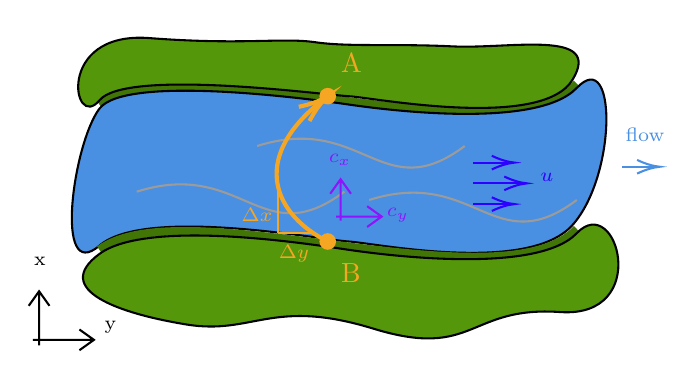
\begin{tikzpicture}[x=0.75pt,y=0.75pt,yscale=-1,xscale=1]
%uncomment if require: \path (0,300); %set diagram left start at 0, and has height of 300

%Curve Lines [id:da608977851192717] 
\draw [color={rgb, 255:red, 65; green, 117; blue, 5 }  ,draw opacity=1 ][line width=3]    (300,110) .. controls (340,80) and (493.51,138.06) .. (530,100) ;
%Shape: Polygon Curved [id:ds9392726871646548] 
\draw  [fill={rgb, 255:red, 74; green, 144; blue, 226 }  ,fill opacity=1 ] (300,112) .. controls (312.68,95.2) and (403.92,107.66) .. (420,110) .. controls (436.08,112.34) and (510.65,122.34) .. (530,102) .. controls (549.35,81.66) and (549.3,143.91) .. (528,168) .. controls (506.7,192.09) and (432.13,176.66) .. (420,176) .. controls (407.87,175.34) and (322.13,158.94) .. (300,178) .. controls (277.87,197.06) and (287.32,128.8) .. (300,112) -- cycle ;
%Curve Lines [id:da6433547723995421] 
\draw [color={rgb, 255:red, 65; green, 117; blue, 5 }  ,draw opacity=1 ][line width=3]    (300,180) .. controls (340,150) and (493.51,208.06) .. (530,170) ;
%Shape: Polygon Curved [id:ds34371397326569686] 
\draw  [fill={rgb, 255:red, 85; green, 151; blue, 11 }  ,fill opacity=1 ] (300,182) .. controls (323.56,164.66) and (403.92,177.66) .. (420,180) .. controls (436.08,182.34) and (510.65,192.34) .. (530,172) .. controls (549.35,151.66) and (566.44,213.06) .. (522,210) .. controls (477.56,206.94) and (481.01,233.06) .. (432,218) .. controls (382.99,202.94) and (374.13,221.23) .. (342,216) .. controls (309.87,210.77) and (276.44,199.34) .. (300,182) -- cycle ;
%Shape: Polygon Curved [id:ds3342416894164969] 
\draw  [fill={rgb, 255:red, 85; green, 151; blue, 11 }  ,fill opacity=1 ] (324,78) .. controls (369.58,81.49) and (387.92,77.66) .. (404,80) .. controls (420.08,82.34) and (442.15,80.63) .. (470,82) .. controls (497.85,83.37) and (542.72,73.49) .. (528,98) .. controls (513.28,122.51) and (432.13,106.66) .. (420,106) .. controls (407.87,105.34) and (312.7,92.51) .. (300,108) .. controls (287.3,123.49) and (278.42,74.51) .. (324,78) -- cycle ;
%Curve Lines [id:da7504908272245701] 
\draw [color={rgb, 255:red, 155; green, 155; blue, 155 }  ,draw opacity=1 ]   (318,152) .. controls (369.01,135.91) and (378,182) .. (418,152) ;
%Curve Lines [id:da01966435364089625] 
\draw [color={rgb, 255:red, 155; green, 155; blue, 155 }  ,draw opacity=1 ]   (376,130) .. controls (427.01,113.91) and (436,160) .. (476,130) ;
%Curve Lines [id:da5498107083025197] 
\draw [color={rgb, 255:red, 155; green, 155; blue, 155 }  ,draw opacity=1 ]   (430,156) .. controls (481.01,139.91) and (490,186) .. (530,156) ;
%Shape: Circle [id:dp01198373160385724] 
\draw  [draw opacity=0][fill={rgb, 255:red, 245; green, 166; blue, 35 }  ,fill opacity=1 ] (406,106) .. controls (406,103.79) and (407.79,102) .. (410,102) .. controls (412.21,102) and (414,103.79) .. (414,106) .. controls (414,108.21) and (412.21,110) .. (410,110) .. controls (407.79,110) and (406,108.21) .. (406,106) -- cycle ;
%Shape: Circle [id:dp6252725126232461] 
\draw  [draw opacity=0][fill={rgb, 255:red, 245; green, 166; blue, 35 }  ,fill opacity=1 ] (406,176) .. controls (406,173.79) and (407.79,172) .. (410,172) .. controls (412.21,172) and (414,173.79) .. (414,176) .. controls (414,178.21) and (412.21,180) .. (410,180) .. controls (407.79,180) and (406,178.21) .. (406,176) -- cycle ;
%Straight Lines [id:da006269855405936053] 
\draw [color={rgb, 255:red, 74; green, 144; blue, 226 }  ,draw opacity=1 ]   (552,140) -- (568,140) ;
\draw [shift={(570,140)}, rotate = 180] [color={rgb, 255:red, 74; green, 144; blue, 226 }  ,draw opacity=1 ][line width=0.75]    (10.93,-3.29) .. controls (6.95,-1.4) and (3.31,-0.3) .. (0,0) .. controls (3.31,0.3) and (6.95,1.4) .. (10.93,3.29)   ;
%Shape: Axis 2D [id:dp579588107341299] 
\draw  (268,223.4) -- (297.36,223.4)(270.94,200) -- (270.94,226) (290.36,218.4) -- (297.36,223.4) -- (290.36,228.4) (265.94,207) -- (270.94,200) -- (275.94,207)  ;
%Curve Lines [id:da1687299064997403] 
\draw [color={rgb, 255:red, 245; green, 166; blue, 35 }  ,draw opacity=1 ][line width=1.5]    (410,176) .. controls (385.7,163.93) and (370.61,137.1) .. (407.67,107.8) ;
\draw [shift={(410,106)}, rotate = 143.13] [color={rgb, 255:red, 245; green, 166; blue, 35 }  ,draw opacity=1 ][line width=1.5]    (14.21,-4.28) .. controls (9.04,-1.82) and (4.3,-0.39) .. (0,0) .. controls (4.3,0.39) and (9.04,1.82) .. (14.21,4.28)   ;
%Straight Lines [id:da5117559499291524] 
\draw [color={rgb, 255:red, 245; green, 166; blue, 35 }  ,draw opacity=1 ]   (386,146) -- (386,172) ;
%Straight Lines [id:da7911427218260162] 
\draw [color={rgb, 255:red, 245; green, 166; blue, 35 }  ,draw opacity=1 ]   (386,172) -- (404,172) ;
%Shape: Axis 2D [id:dp020929963075495994] 
\draw [color={rgb, 255:red, 144; green, 19; blue, 254 }  ,draw opacity=1 ] (414,164) -- (436,164)(416.2,146) -- (416.2,166) (429,159) -- (436,164) -- (429,169) (411.2,153) -- (416.2,146) -- (421.2,153)  ;
%Straight Lines [id:da5963450198567739] 
\draw [color={rgb, 255:red, 46; green, 0; blue, 255 }  ,draw opacity=1 ]   (480,148) -- (504,148) ;
\draw [shift={(506,148)}, rotate = 180] [color={rgb, 255:red, 46; green, 0; blue, 255 }  ,draw opacity=1 ][line width=0.75]    (10.93,-3.29) .. controls (6.95,-1.4) and (3.31,-0.3) .. (0,0) .. controls (3.31,0.3) and (6.95,1.4) .. (10.93,3.29)   ;
%Straight Lines [id:da016477493607424232] 
\draw [color={rgb, 255:red, 46; green, 0; blue, 255 }  ,draw opacity=1 ]   (480,158) -- (498,158) ;
\draw [shift={(500,158)}, rotate = 180] [color={rgb, 255:red, 46; green, 0; blue, 255 }  ,draw opacity=1 ][line width=0.75]    (10.93,-3.29) .. controls (6.95,-1.4) and (3.31,-0.3) .. (0,0) .. controls (3.31,0.3) and (6.95,1.4) .. (10.93,3.29)   ;
%Straight Lines [id:da8245950958515168] 
\draw [color={rgb, 255:red, 46; green, 0; blue, 255 }  ,draw opacity=1 ]   (480,138) -- (498,138) ;
\draw [shift={(500,138)}, rotate = 180] [color={rgb, 255:red, 46; green, 0; blue, 255 }  ,draw opacity=1 ][line width=0.75]    (10.93,-3.29) .. controls (6.95,-1.4) and (3.31,-0.3) .. (0,0) .. controls (3.31,0.3) and (6.95,1.4) .. (10.93,3.29)   ;

% Text Node
\draw (415,84) node [anchor=north west][inner sep=0.75pt]  [color={rgb, 255:red, 245; green, 166; blue, 35 }  ,opacity=1 ] [align=left] {A};
% Text Node
\draw (415,185) node [anchor=north west][inner sep=0.75pt]  [color={rgb, 255:red, 245; green, 166; blue, 35 }  ,opacity=1 ] [align=left] {B};
% Text Node
\draw (552,120) node [anchor=north west][inner sep=0.75pt]  [color={rgb, 255:red, 74; green, 144; blue, 226 }  ,opacity=1 ] [align=left] {{\scriptsize flow}};
% Text Node
\draw (267,182) node [anchor=north west][inner sep=0.75pt]  [color={rgb, 255:red, 0; green, 0; blue, 0 }  ,opacity=1 ] [align=left] {{\scriptsize x}};
% Text Node
\draw (301,213) node [anchor=north west][inner sep=0.75pt]  [color={rgb, 255:red, 0; green, 0; blue, 0 }  ,opacity=1 ] [align=left] {{\scriptsize y}};
% Text Node
\draw (385,176.4) node [anchor=north west][inner sep=0.75pt]  [font=\scriptsize]  {$\textcolor[rgb]{0.96,0.65,0.14}{\Delta y}$};
% Text Node
\draw (367,158.4) node [anchor=north west][inner sep=0.75pt]  [font=\scriptsize]  {$\textcolor[rgb]{0.96,0.65,0.14}{\Delta x}$};
% Text Node
\draw (409,132.4) node [anchor=north west][inner sep=0.75pt]  [font=\scriptsize,color={rgb, 255:red, 144; green, 19; blue, 254 }  ,opacity=1 ]  {$\textcolor[rgb]{0.56,0.07,1}{c_{x}}$};
% Text Node
\draw (437,158.4) node [anchor=north west][inner sep=0.75pt]  [font=\scriptsize,color={rgb, 255:red, 144; green, 19; blue, 254 }  ,opacity=1 ]  {$\textcolor[rgb]{0.56,0.07,1}{c_{y}}$};
% Text Node
\draw (511,141.4) node [anchor=north west][inner sep=0.75pt]  [font=\scriptsize,color={rgb, 255:red, 144; green, 19; blue, 254 }  ,opacity=1 ]  {$\textcolor[rgb]{0.18,0,1}{u}$};


\end{tikzpicture}



    \caption{Fluss, der überquert werden soll. Die Strömungsgeschwindigkeit \(u\) ist dunkelblau eingezeichnet und bezieht sich auf die Geschwindigkeit des Flusses. Dabei ist zu beachten, dass diese nicht überall im Fluss gleich sein muss; sie könnte zum Ufer hin langsamer und in der Mitte des Flusses schneller sein. Somit ist sie von \(x\) abhängig. \(c_x\) und \(c_y\) bezeichnen die Geschwindigkeiten in \(x\)- und \(y\)-Richtung der schwimmenden Person. \(\Delta x\) und \(\Delta y\) sind die sehr kleinen Distanzen auf der Strecke von A nach B.
    \label{fig:river_dif}}
\end{figure}

\textbf{Zeitoptimierung} Die Zeit \(T\), die für die Flussüberquerung benötigt wird, kann mittels
\[
T = \int \frac{1}{v} \, ds
\]
berechnet werden, wobei \(v\) die Geschwindigkeit ist und \(s\) die dabei zurückgelegte Strecke.

\textbf{Zeit für ein Streckenstück} Die Zeit, die für ein sehr kleines Streckenstück benötigt wird, kann ermittelt werden, indem man diese kleine Strecke durch die Geschwindigkeit auf dieser kleinen Strecke teilt. Dies sieht so aus:
\begin{equation}\label{eq:time_for_distance_pice}
    \frac{ds}{\sqrt{(c_y - u)^2 + c_x^2}}
\end{equation}
wobei \(u\) die Geschwindigkeit des Flusses bzw. der Strömung an dieser Stelle im Fluss ist. \(c_x\) und \(c_y\) bezeichnen die Geschwindigkeiten der schwimmenden Person in \(x\)- und \(y\)-Richtung. Eine grafische Darstellung ist in Abbildung \ref{fig:river_dif} zu sehen.

\textbf{Zeit für die Strömungskompensation} Die Zeit, die zusätzlich zur Flussüberquerung benötigt wird, um die Strömung zu kompensieren, ist definiert als 
\begin{equation}\label{eq:time_compenation}
    \frac{dx}{u}
\end{equation}

\textbf{Gesamte Zeit} Die gesamte Zeit für ein sehr kleines Streckenstück kann mittels der Gleichungen \ref{eq:time_for_distance_pice} und \ref{eq:time_compenation} hergeleitet werden. Es folgt:
\begin{equation}\label{eq:time_pice_total}
    \frac{dx}{u} + \frac{ds}{\sqrt{(c_y - u)^2 + c_x^2}}
\end{equation}

\textbf{Strecke}
Für allgemeine Fälle kann die Distanz einer Strecke mit der Formel
\[
ds = \sqrt{\Delta x^2 + \Delta y^2} \approx \sqrt{1 + y'^2} \, dx
\]
angenähert werden, wobei sich die Variablen wieder auf Abbildung \ref{fig:river_dif} beziehen.

\textbf{Integral} Nun ist es an der Zeit, ein Integral für die Zeit, die benötigt wird, um den Fluss zu überqueren, aufzustellen, basierend auf den obigen Formeln. Das Integral:
\begin{equation}\label{eq:integral_time}
    T = \int L(x, y, y') \, dx = \int \left( \frac{1}{u} + \frac{\sqrt{1 + y'^2}}{\sqrt{(c_y - u)^2 + c_x^2}} \right) dx
\end{equation}
soll für eine möglichst kleine Zeit \(T\) optimiert werden, um die energieeffizienteste Überquerung zu erreichen.

\textbf{Lagrange-Funktion} Aus dem Lagrange-Integral \ref{eq:integral_time} kann die Lagrange-Funktion
\begin{equation}\label{eq:lagrange_integral}
    L(x, y, y') = \frac{1}{u} + \frac{\sqrt{1 + y'^2}}{\sqrt{(c_y - u)^2 + c_x^2}}
\end{equation}
herausgelesen werden. Die Lagrange-Funktion wird für das Variationsprinzip benötigt, um die Funktion für die energieeffizienteste Methode für die Flussüberquerung zu berechnen.

\textbf{Euler-Lagrange-Gleichung} Die Euler-Lagrange-Gleichung kann vereinfacht werden, da sie nicht direkt von \(y\) abhängig ist. Die Ableitungen der Lagrange-Funktion sind:
\begin{equation}\label{eq:Lagrange_derivites_1}
    \frac{\partial L}{\partial y'} = \text{constant}
\end{equation}
\begin{multline}\label{eq:Lagrange_derivites_2}
    \frac{\partial L}{\partial y'} = \frac{\partial}{\partial y'} \left( \frac{1}{u} + \frac{\sqrt{1 + y'^2}}{\sqrt{(c_y - u)^2 + c_x^2}} \right) \\
    = \frac{1}{\sqrt{(c_y - u)^2 + c_x^2}} \cdot \frac{y'}{\sqrt{1 + y'^2}} = \text{constant} = \frac{1}{g}
\end{multline}
Auflösung nach \(y'\):
\begin{align}
    y' &= \sqrt{(c_y - u)^2 + c_x^2} \cdot \sqrt{1 + y'^2} \cdot \frac{1}{g} \\
    y' &= \sqrt{\frac{c_y^2 - 2 \cdot c_y \cdot u + u^2 + c_x^2}{g^2 - c_y^2 + 2 \cdot c_y \cdot u - u^2 - c_x^2}}\label{eq:angle}
\end{align}
Wird das Integral über \(y'\) gebildet, erhält man die Zeit:
\begin{equation}\label{eq:time_integral}
    T = y = \int \sqrt{\frac{c_y^2 - 2 \cdot c_y \cdot u + u^2 + c_x^2}{g^2 - c_y^2 + 2 \cdot c_y \cdot u - u^2 - c_x^2}} \, dx
\end{equation}





















        

%     \caption{Fluss der überquert werden soll. Die Strömungsgeschwindigkeit \(u\) dunkelblau eingezeichnet beziht sich auf die geschwindigkeit des Flusses, dabei ist zu beachten das diese nicht überal im Fluss gleich sein muss, sie könnte zum Ufer des Flusses hin langamer sein und in der mitte des Flusses schneller. Somit ist sie von \(x\) abhängig. \(c_x\)} und \(c_y\) bezeichenen die Geschwindigkeiten in \(x\)- und \(y\)-Richtung der schwimmenden Person. \(\Delta x\) und \(\Delta y\) sind die sehr kleinen Distanzen auf der Strecke von A nach B.
%     \label{fig:river_dif}
% \end{figure}


% \textbf{Zeitoptimierung} Die Zeit \(T\) die Für die Flussüberquerung gebraucht wird kann mittels \[T=\int{\frac{1}{v}ds}\] berechnet werden, wobei \(v\) die Geschwindigkeit ist und \(s\) die dabei zurückgelegte Strecke. 

% \textbf{Zeit für ein Streckenstück} Die Zeit die für ein sehr kleines streckenstück benötigt wird kann ermittelt werden in dem man diese kleine Strecke durch die Geschwindigkeit auf dieser kleinen strecke teilt. Dies sith so aus:
% \begin{equation}\label{eq:time_for_distance_pice}
%     \frac{ds}{\sqrt{(c_y-u)^2+c_x^2}}
% \end{equation}
% Wobei \(u\) die geschwindigkeit des Flsses bzw. der Strömung and dieser Stelle im Fluss ist. \(c_x\) und \(c_y\) bezeichen die Geschwindigkeiten der schwimmenden Person in Axenrichtung in \(x\) und \(y\) richtung, eine Graphische darstellung ist in Abbildung \ref{fig:river_dif} dargestellt.

% \textbf{Zeit für die Strömungskompensation} Die Zeit die zusätzlich zur Flussüberquerung bebraucht wird um die Strömung zu kompensieren ist definiert als 
% \begin{equation}\label{eq:time_compenation}
%     \frac{dx}{u}
% \end{equation}

% \textbf{Gesamte Zeit} Die gesmate Teit für ein sehr kleines Streckenstück kann mitels den Gleicungen \ref{eq:time_for_distance_pice} und \ref{eq:time_compenation} hergeleitet werden, es folgt: 
% \begin{equation}\label{eq:time_pice_total}
%     \frac{dx}{u} + \frac{ds}{\sqrt{(c_y-u)^2+c_x^2}}.
% \end{equation}


% \textbf{Strecke}
% Für allgemeine Fälle kann die Distanz einer Strecke mit der Formel
% \begin{equation}
%     ds=\sqrt{\Delta x^2 + \Delta y^2} \approx \sqrt{1+y'^2}dx
% \end{equation}
% angenähert werden, wobei sich die Variabeln wider auf Abbildung \ref{fig:river_dif} bezihn. 

% \textbf{Integral} Nun ist es so weit das ein Integral für die Zeit die gebraucht wird um den Fluss zu überqueren aufgestellt werden kann, mit den Formeln von oben. Das Integral:
% \begin{equation}\label{eq:integral_time}
%     T=\int L(x,y,y')dx = \int\frac{1}{u} + \frac{\sqrt{1+y'^2}}{\sqrt{(c_y-u)^2+c_x^2}}dx
% \end{equation}
% soll für eine möglischst kleine Zeit \(T\) optimiert werden um die energieefizientiste überquerung zu bekommen

% \textbf{Lagrange-Funktion} Aus dem Langrange-Integral \ref{eq:integral_time} kann die Lagrange Funktion 
% \begin{equation}\label{eq:lagrange_integral}
%     L(x,y,y')dx = \frac{1}{u} + \frac{\sqrt{1+y'^2}}{\sqrt{(c_y-u)^2+c_x^2}}dx
% \end{equation}
% herausgelesen werden. Die Lagrange-Funtion wird für das Variationsprinzip gebraucht um die Funktion für die Energieefizäntiste Methode für die Flussüberquerung zu berechnen.


% \textbf{Euler-Lagrange Formel} Euler-Lagrange Formel kann vereinfacht werden da sie nicht direkt von \(y\) abhägig ist. Ableitungen von der Lagrange-Funktion:
% \begin{equation}\label{eq:Lagrange_derivites_1}
%     \frac{\partial L}{\partial y'}=constant
% \end{equation}
% \begin{multline}\label{eq:Lagrange_derivites_2}
%     \frac{\partial L}{\partial y'}=\frac{\partial}{\partial y'}\frac{1}{u}+\frac{\sqrt{1+y'^2}}{\sqrt{(c_y-u)^2+c_x^2}}\\
%     =\frac{1}{\sqrt{(c_y-u)^2+c_x^2}}\frac{y'}{\sqrt{1+y'^2}}=constant=\frac{1}{g}
% \end{multline}\label{eq:Lagrange_derivites_y'}
% nach \(y'\) auflössen
% \begin{align}
%     y'&=\sqrt{(c_y-u)^2+c_x^2}\cdot\sqrt{1+y'^2}\cdot\frac{1}{g} \\
%     y'&=\sqrt{\frac{c_y^2-2\cdot c_y\cdot u+u^2+c_x^2}{g^2-c_y^2+2\cdot c_y\cdot u-u^2-c_x^2}}\label{eq:angle}
% \end{align}
% Bildet man das Integral um \(y'\) bekommt man die Zeit
% \begin{equation}\label{eq:time_integral}
%     T=y=\int\sqrt{\frac{c_y^2-2\cdot c_y\cdot u+u^2+c_x^2}{g^2-c_y^2+2\cdot c_y\cdot u-u^2-c_x^2}}dx
% \end{equation}





